\chapter{Introduction} \label{ChapIntroduction}
GIRAF is a series of applications(apps) for Android, intended to help citizens with autism in their everyday life. Over the past four years GIRAF have been developed by students at Aalborg University, with a new group of students taking the mantle every year. As a result of this, it was hard to get an overview of the project in its entirety. We here give an overview of the GIRAF project as it was, when we started working on it, and we also give some insight into the organization of the project.

\section{Status of GIRAF} %To add: pictures to help descripe apps.
Overall GIRAF is in a somewhat functional state with several problems ranging from small to severe regarding stability, reliability, and usability.
GIRAF is published in Google's Play Store with the individual apps being version 1.0, while the launcher-app, the main app the other apps should be executed from, is version 2.2. The version-numbering is not entirely correct, as some of the apps does not function correctly yet and as such they should not have been published as official versions but rather as alpha or beta versions. The majority of the apps does function correctly, but only a few of them are ready for public release.
Google Analytics was incorporated in roughly one third of the apps, with between three and six months of data on usage and crashes being available for these apps. The data has been gathered since the newest version of the apps were published, in general since the 25th of August 2014.

\section{Multiproject, Subprojects, and Responsibility} %To add better description of Scrum of Scrums principle.
The overall goal for the multiproject this year was, to make a working system that is usable and stable. A multiproject in this context being an overall project that several groups, in this case all 6th semester software groups, work on in collaboration. In order to achieve a better workflow, the project was split into three subprojects: Database (DB), Graphical User Interface(GUI), and Build and Deployment(B\&D). Our group were a part of B\&D, along with 3 other groups. Both the DB and GUI subprojects had 5 groups each. See Figure \ref{ScrumOfScrumsOverview} for an overview of the structure of this years multiproject.

\begin{figure}
	\centering
	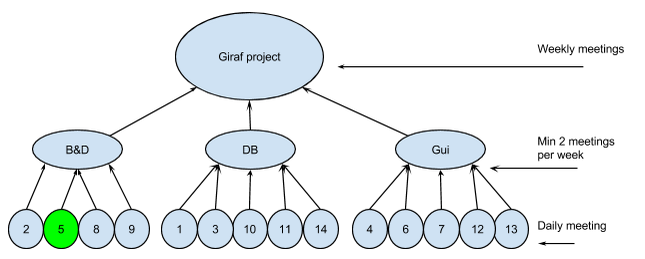
\includegraphics[width=0.8 \textwidth]{pictures/ScrumOfScrum.png}
	\caption{Overview of the project structure with subprojects and the individual groups depicted, our group is marked with green.}
	\label{ScrumOfScrumsOverview}
\end{figure}

\subsection{Database}
DB groups were responsible for handling all things database related, this included making current data accessible and adding new data to the database, as per request from other groups or as needed.

\subsection{Graphical User Interface}
GUI groups were mainly responsible for developing the different apps, this included making general changes in the apps and bug fixing anything related to the apps.

\subsection{Build and Deployment}
B\&D groups were responsible for most of the internal project matters, this included maintaining the server services, developing and maintaining the automatic build tools, handling publication of the apps, and administrating the version control.

\section{Project organization}
The project is organized using Scrum principles where the individual subprojects held Scrum of Scrum meetings twice a week. The individual groups can follow any principles that they would like, but Scrum was recommended. Our group decided to follow Scrum to have the same structure as the project.
In addition an overall meeting was held every week where at least one representative from each group were present. At these meetings the overall status for each subproject were given, and any decisions that needed overall consensus were discussed.

As the overall structure is Scrum, the project was split into four sprints. The first sprint was devoted to bug fixing, user stories and tasks that were still unsolved from last year, and setting up and organizing project tools. In regards to user stories, it was decided early on at an overall meeting, to operate with two types of user stories, those from the costumers, these were called user stories; and those from the other groups, called developer stories. For consistencies sake we will just refer to both as user stories in the report, as the difference was mainly a concern when groups from different subprojects where discussing internally.

%Something about the organization of sprintends will be written here.
